\documentclass[10pt]{article}
\usepackage{tikz}
\usetikzlibrary{positioning,fit,arrows.meta,calc}
\usepackage[paperwidth=8in,paperheight=4.5in,margin=0.3in]{geometry}

\begin{document}
\thispagestyle{empty}
\pagestyle{empty}

\centering
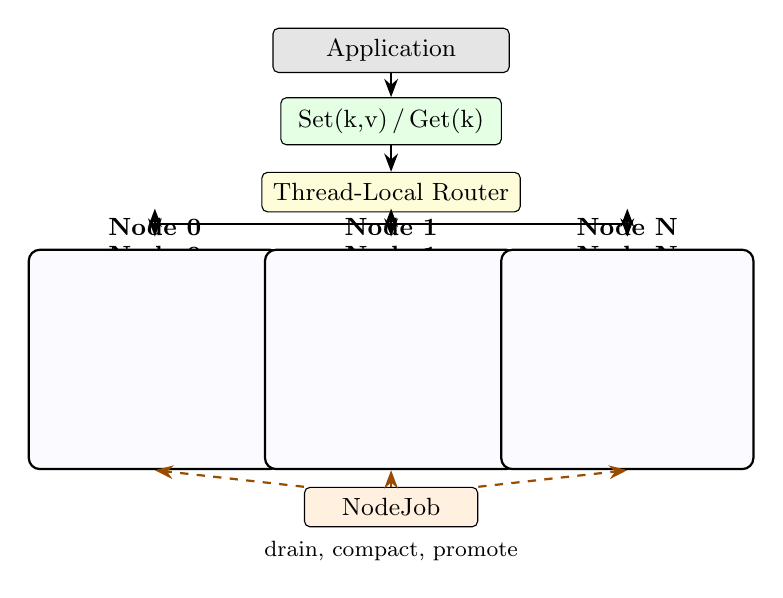
\begin{tikzpicture}[
    >=Stealth,
    every node/.style={font=\small},
    block/.style={draw, rounded corners=2pt, minimum height=0.5cm, align=center, inner sep=4pt},
]

% Row 0 (y=0): Application
\node[block, fill=gray!20, minimum width=3cm] (app) at (0,0) {Application};

% Row 1 (y=-0.9): API
\node[block, fill=green!10, minimum width=2.8cm] (api) at (0,-0.9) {Set(k,v)\,/\,Get(k)};
\draw[->,thick] (app) -- (api);

% Row 2 (y=-1.8): Router
\node[block, fill=yellow!15, minimum width=2.8cm] (router) at (0,-1.8) {Thread-Local Router};
\draw[->,thick] (api) -- (router);

% Node X positions
\def\nodexA{-3.0}
\def\nodexB{0}
\def\nodexC{3.0}

% Row 3 (y=-2.6): Node labels
\node[font=\small\bfseries] (n0lab) at (\nodexA,-2.6) {Node 0};
\node[font=\small\bfseries] (n1lab) at (\nodexB,-2.6) {Node 1};
\node[font=\large] (dots) at (1.5,-2.6) {$\cdots$};
\node[font=\small\bfseries] (nNlab) at (\nodexC,-2.6) {Node N};

% Arrows from router to labels (pointing DOWN)
\draw[->,thick] (router.south) -- ++(0,-0.15) -| (n0lab.north);
\draw[->,thick] (router.south) -- (n1lab.north);
\draw[->,thick] (router.south) -- ++(0,-0.15) -| (nNlab.north);

% Row 4 (y=-3.1): CMap
\node[block, fill=teal!10, minimum width=1.6cm] (cmap0) at (\nodexA,-3.1) {CMap};
\node[block, fill=teal!10, minimum width=1.6cm] (cmap1) at (\nodexB,-3.1) {CMap};
\node[block, fill=teal!10, minimum width=1.6cm] (cmapN) at (\nodexC,-3.1) {CMap};

% Row 5 (y=-3.65): ARC
\node[block, fill=red!8, minimum width=1.6cm] (arc0) at (\nodexA,-3.65) {ARC};
\node[block, fill=red!8, minimum width=1.6cm] (arc1) at (\nodexB,-3.65) {ARC};
\node[block, fill=red!8, minimum width=1.6cm] (arcN) at (\nodexC,-3.65) {ARC};

% Row 6 (y=-4.2): SpinLock
\node[block, fill=purple!8, minimum width=1.6cm] (lock0) at (\nodexA,-4.2) {SpinLock};
\node[block, fill=purple!8, minimum width=1.6cm] (lock1) at (\nodexB,-4.2) {SpinLock};
\node[block, fill=purple!8, minimum width=1.6cm] (lockN) at (\nodexC,-4.2) {SpinLock};

% Row 7 (y=-4.75): Pages (as a single block representing the page pool)
\node[block, fill=blue!12, minimum width=1.6cm] (pages0) at (\nodexA,-4.75) {Pages + Staging};
\node[block, fill=blue!12, minimum width=1.6cm] (pages1) at (\nodexB,-4.75) {Pages + Staging};
\node[block, fill=blue!12, minimum width=1.6cm] (pagesN) at (\nodexC,-4.75) {Pages + Staging};

% Node boxes (enclose CMap through Pages)
\node[draw, thick, rounded corners=4pt, inner sep=8pt, fill=blue!2,
      fit=(cmap0)(arc0)(lock0)(pages0)] (n0box) {};
\node[draw, thick, rounded corners=4pt, inner sep=8pt, fill=blue!2,
      fit=(cmap1)(arc1)(lock1)(pages1)] (n1box) {};
\node[draw, thick, rounded corners=4pt, inner sep=8pt, fill=blue!2,
      fit=(cmapN)(arcN)(lockN)(pagesN)] (nNbox) {};

% Move node labels to top of boxes
\node[font=\small\bfseries, above=0.04cm of n0box.north] (n0lab2) {Node 0};
\node[font=\small\bfseries, above=0.04cm of n1box.north] (n1lab2) {Node 1};
\node[font=\small\bfseries, above=0.04cm of nNbox.north] (nNlab2) {Node N};

% Fix arrows to point to node box tops
\draw[->,thick] (router.south) -- ++(0,-0.15) -| (n0lab2.north);
\draw[->,thick] (router.south) -- (n1lab2.north);
\draw[->,thick] (router.south) -- ++(0,-0.15) -| (nNlab2.north);

% Row 8 (y=-5.8): NodeJob
\node[block, fill=orange!12, minimum width=2.2cm] (nodejob) at (\nodexB,-5.8) {NodeJob};
\node[font=\footnotesize, below=0.05cm of nodejob.south] (mainttext) {drain, compact, promote};

% Dashed arrows from NodeJob to each node box
\draw[->,dashed,thick,orange!60!black] (nodejob.north) -- (n1box.south);
\draw[->,dashed,thick,orange!60!black] (nodejob.north west) -- (n0box.south);
\draw[->,dashed,thick,orange!60!black] (nodejob.north east) -- (nNbox.south);

\end{tikzpicture}

\end{document}
